\documentclass[a4paper]{article}
%\VignetteIndexEntry{Short manual for the chemCal package}
\usepackage{hyperref}

\title{Basic calibration functions for analytical chemistry}
\author{Johannes Ranke}

\usepackage{/usr/share/R/share/texmf/Sweave}
\begin{document}
\maketitle

When calibrating an analytical method, the first task is to generate
a suitable model. If we want to use the \texttt{chemCal} functions, we
will have to restrict ourselves to univariate, possibly weighted
\footnote{
For the weighted case, the function \texttt{predict.lm} would have to be 
adapted (Bug report PR\#8877), in order to allow for weights for the x values
used to predict the y values. This affects the functions \texttt{calplot}
and \texttt{lod}.
}, linear regression so far.

Once such a model has been created, the calibration can be graphically
shown by using the \texttt{calplot} function:

\begin{Schunk}
\begin{Sinput}
> library(chemCal)
> data(massart97ex3)
> attach(massart97ex3)
> m0 <- lm(y ~ x)
> calplot(m0)
\end{Sinput}
\end{Schunk}
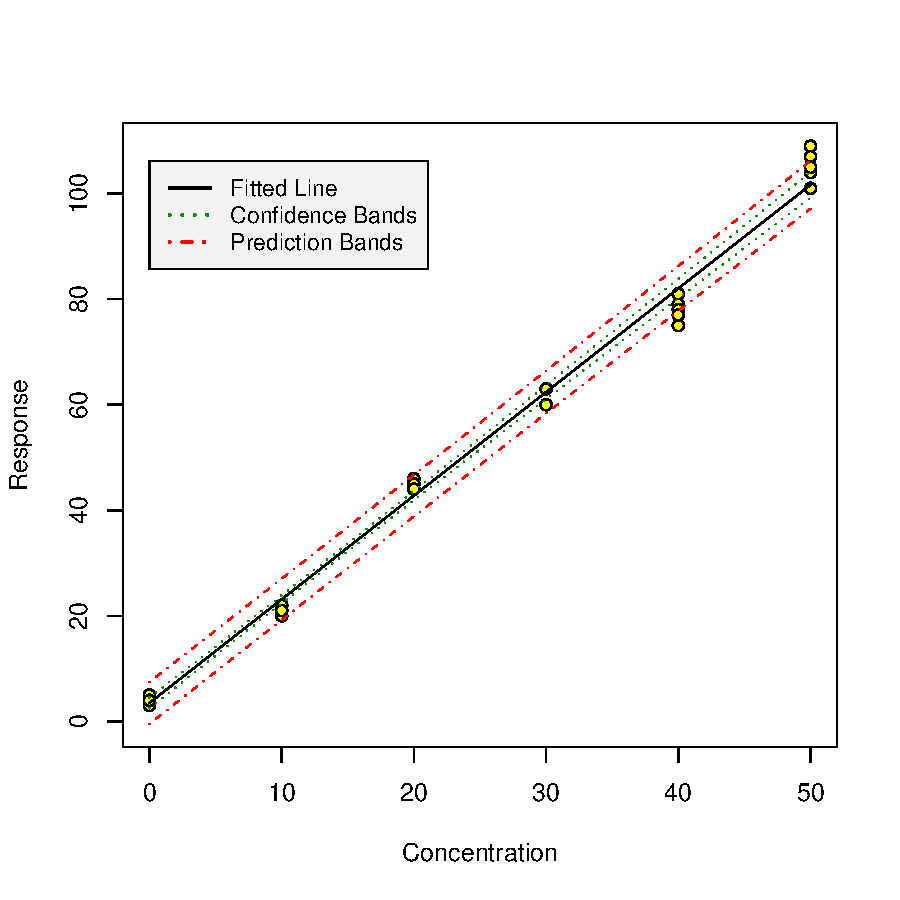
\includegraphics{chemCal-001}

As we can see, the scatter increases with increasing x. This is also
illustrated by one of the diagnostic plots for linear models 
provided by R: 

\begin{Schunk}
\begin{Sinput}
> plot(m0, which = 3)
\end{Sinput}
\end{Schunk}
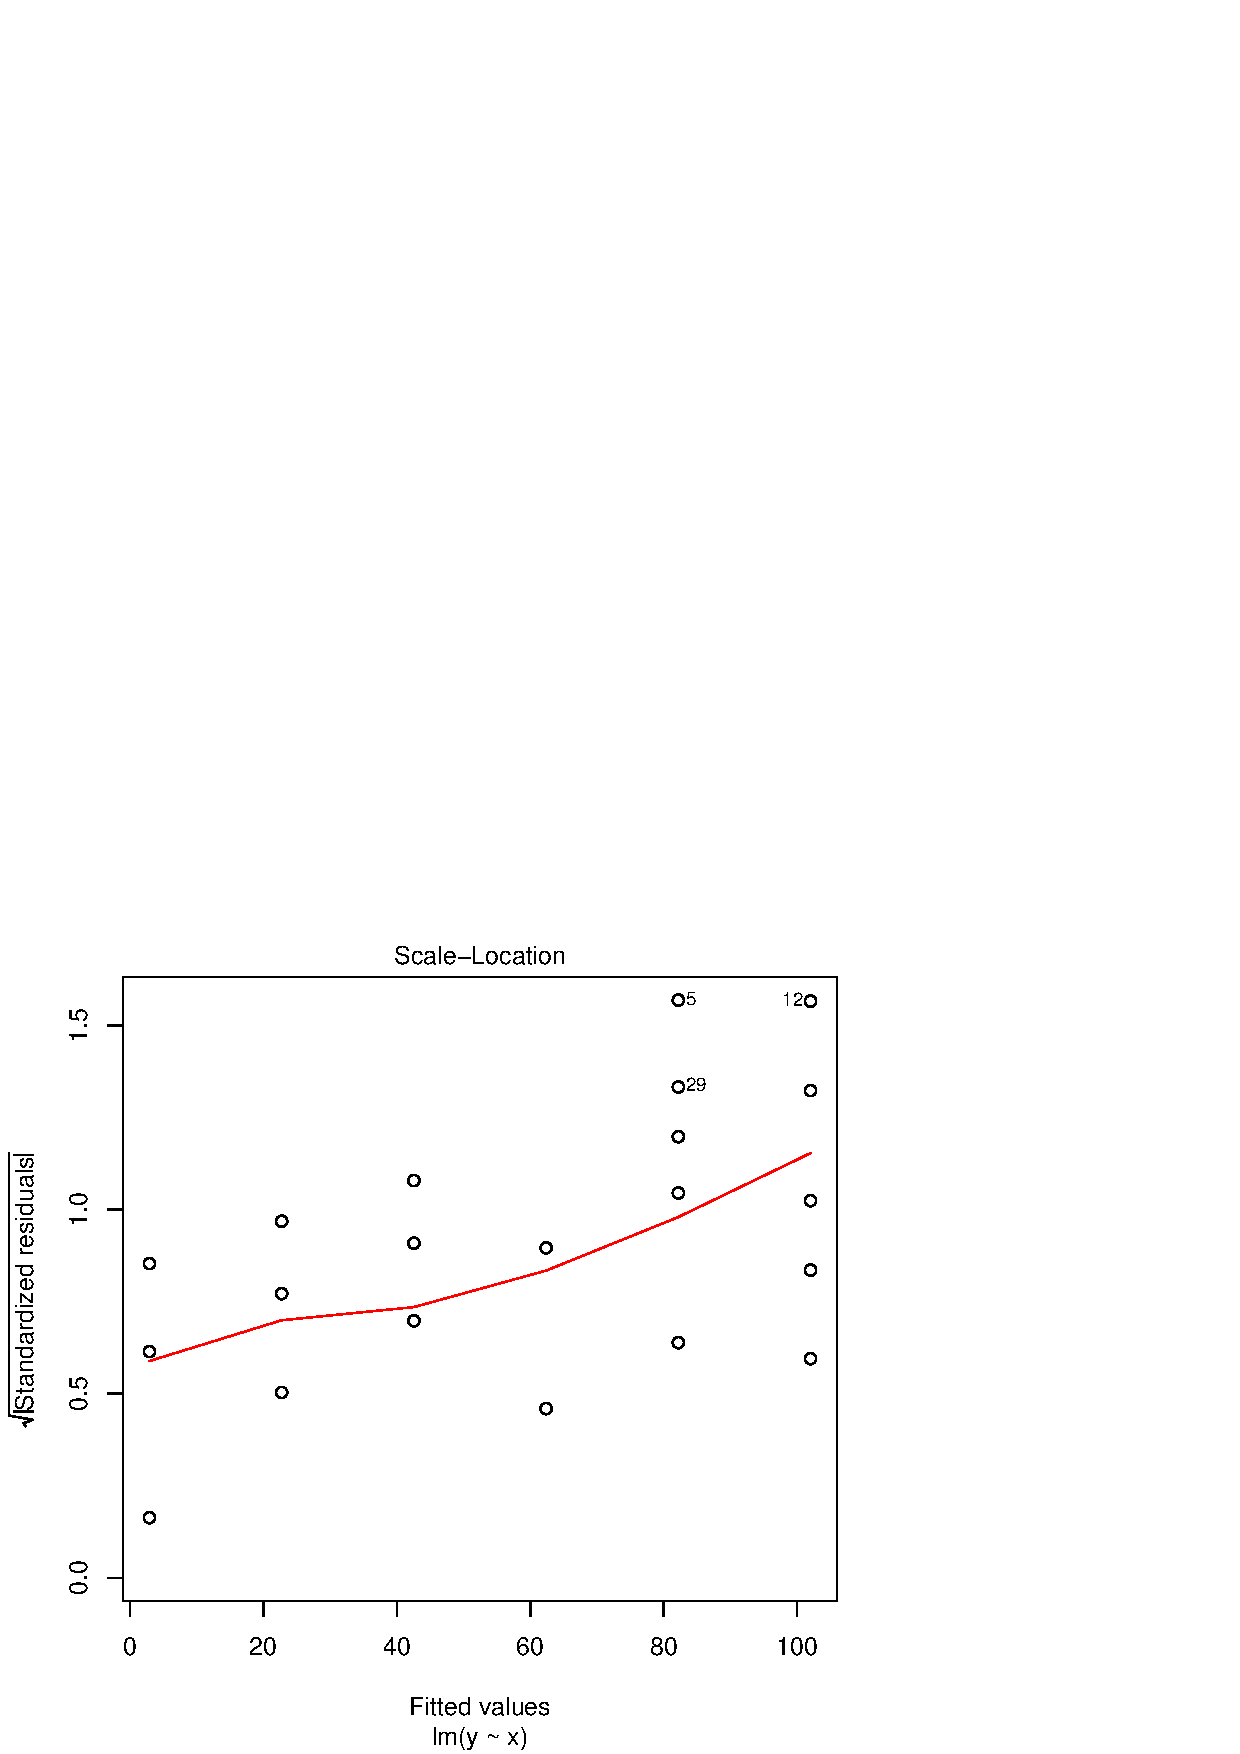
\includegraphics{chemCal-002}

Therefore, in Example 8 in \cite{massart97} weighted regression
is proposed which can be reproduced by

\begin{Schunk}
\begin{Sinput}
> yx <- split(y, x)
> ybar <- sapply(yx, mean)
> s <- round(sapply(yx, sd), digits = 2)
> w <- round(1/(s^2), digits = 3)
> weights <- w[factor(x)]
> m <- lm(y ~ x, w = weights)
\end{Sinput}
\end{Schunk}

Unfortunately, \texttt{calplot} does not work on weighted linear models,
as noted in the footnote above.

If we now want to predict a new x value from measured y values,
we use the \texttt{inverse.predict} function:

\begin{Schunk}
\begin{Sinput}
> inverse.predict(m, 15, ws = 1.67)
\end{Sinput}
\begin{Soutput}
$Prediction
[1] 5.865367

$`Standard Error`
[1] 0.7288138

$Confidence
[1] 2.023511

$`Confidence Limits`
[1] 3.841856 7.888878
\end{Soutput}
\begin{Sinput}
> inverse.predict(m, 90, ws = 0.145)
\end{Sinput}
\begin{Soutput}
$Prediction
[1] 44.06025

$`Standard Error`
[1] 2.310001

$Confidence
[1] 6.41359

$`Confidence Limits`
[1] 37.64666 50.47384
\end{Soutput}
\end{Schunk}

The weight \texttt{ws} assigned to the measured y value has to be 
given by the user in the case of weighted regression. By default, 
the mean of the weights used in the linear regression is used.

\section*{Theory for \texttt{inverse.predict}}
Equation 8.28 in \cite{massart97} gives a general equation for predicting the
standard error $s_{\hat{x_s}}$ for an x value predicted from measurements of y
according to the linear calibration function $ y = b_0 + b_1 \cdot x$:

\begin{equation}
s_{\hat{x_s}} = \frac{s_e}{b_1} \sqrt{\frac{1}{w_s m} + \frac{1}{\sum{w_i}} +
    \frac{(\bar{y_s} - \bar{y_w})^2 \sum{w_i}}
        {{b_1}^2 \left( \sum{w_i} \sum{w_i {x_i}^2} - 
            {\left( \sum{ w_i x_i } \right)}^2 \right) }}
\end{equation}

with

\begin{equation}
s_e = \sqrt{ \frac{\sum w_i (y_i - \hat{y_i})^2}{n - 2}}
\end{equation}

where $w_i$ is the weight for calibration standard $i$, $y_i$ is the mean $y$
value (!) observed for standard $i$, $\hat{y_i}$ is the estimated value for
standard $i$, $n$ is the number calibration standards, $w_s$ is the weight
attributed to the sample $s$, $m$ is the number of replicate measurements of
sample $s$, $\bar{y_s}$ is the mean response for the sample, 
$\bar{y_w} = \frac{\sum{w_i y_i}}{\sum{w_i}}$ is the weighted mean of responses
$y_i$, and $x_i$ is the given $x$ value for standard $i$.

The weight $w_s$ for the sample should be estimated or calculated in accordance
to the weights used in the linear regression. 

I adjusted the above equation in order to be able to take a different
precisions in standards and samples into account. In analogy to Equation 8.26
from \cite{massart97} we get

\begin{equation}
s_{\hat{x_s}} = \frac{1}{b_1} \sqrt{\frac{{s_s}^2}{w_s m} + 
    {s_e}^2 \left( \frac{1}{\sum{w_i}} +
        \frac{(\bar{y_s} - \bar{y_w})^2 \sum{w_i}}
            {{b_1}^2 \left( \sum{w_i} \sum{w_i {x_i}^2} - {\left( \sum{ w_i x_i } \right)}^2 \right) } \right) }
\end{equation}

\begin{thebibliography}{1}
\bibitem{massart97}
Massart, L.M, Vandenginste, B.G.M., Buydens, L.M.C., De Jong, S., Lewi, P.J.,
Smeyers-Verbeke, J. 
\newblock Handbook of Chemometrics and Qualimetrics: Part A,
\newblock Elsevier, Amsterdam, 1997
\end{thebibliography}

\end{document}
